\begin{frame}
    \centering
    \begin{figure}[H]
        
\includegraphics[keepaspectratio, width=0.7\paperwidth, height=\paperheight]{LeeLogo}
    \end{figure}
    Informatik: Programmieren\\
    Lektion 02 \emoji{nerd-face}: \textbf{Neue Befehle definieren}
\end{frame}

\begin{frame}[fragile]{Neue Befehle definieren}
\begin{lstlisting}[style=TigerJython,escapechar=!]
from gturtle import *
makeTurtle()

def quadrat():
    repeat 4:
        fd(100)
        rt(90)

quadrat() !\tikzmark{to1}!
rt(45)
quadrat() !\tikzmark{to2}!
\end{lstlisting}
\begin{itemize}
\item Definition = \lstinline[style=TigerJython]|def| = Funktion
\item Ähnlich einem Kochrezept
\begin{itemize}
\item Beschreibung der auzuführenden Schritte
\item Wird erst ausgeführt, sobald auf\tikzmark{from}gerufen! 
\end{itemize}
\only<2->{
\begin{tikzpicture}[overlay,remember picture]
\draw[red,-stealth] (from.north) to[bend right] (to1);
\draw[red,-stealth] (from.north) to[bend right] (to2);
\end{tikzpicture}}
\end{itemize}
\end{frame}

\begin{frame}[fragile]{Neue Befehle definieren}
\scriptsize
\begin{columns}
\begin{column}{.4\textwidth}
\begin{lstlisting}[style=TigerJython,escapechar=!]
from gturtle import *
makeTurtle()
hideTurtle()

def viereck():
    repeat 4:
        fd(100)
        rt(360/4)

def viereck_blume():
    repeat 10:
        viereck()
        rt(360/10)

viereck_blume()
\end{lstlisting}
\begin{figure}[H]
\centering
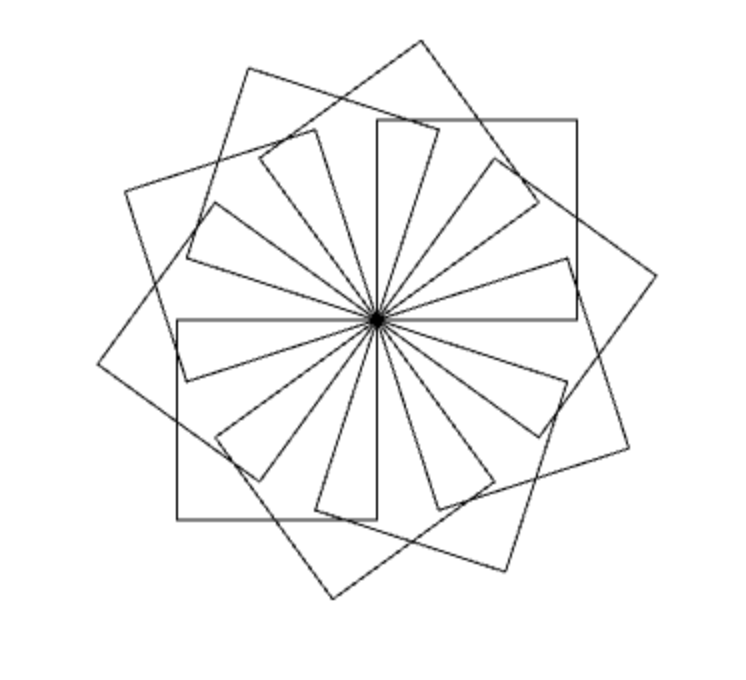
\includegraphics[width=0.6\columnwidth]{GrundlagenInfo/Programmieren/Figures/viereck_blume}
\end{figure}
\end{column}
\begin{column}{.5\textwidth}
\normalsize
\begin{itemize}
\item \textbf{Modularität}: Zerlegung des Programms in kleinere Stücke
\item \textbf{Übersichtlicher}!
\end{itemize}
\end{column}
\end{columns}
\end{frame}

\begin{frame}[fragile]{Auftrag}
\begin{itemize}
\item \aufgabebox{Aufgaben 2.1 - 2.7}
\item \abgabebox{Abgabe auf Moodle: 2.7}
\item \aufgabebox{Aufgaben 2.8 - 2.18}
\item \abgabebox{Abgabe auf Moodle: 2.10}
\end{itemize}
\end{frame}